\section{Scheduling}
\subsection{Statisch/Dynamisch}
\begin{itemize}
	\item Statisch
	\begin{itemize}
		\item ``Fahrplan`` im vorhinein festlegen
		\item Einsatz: Zyklische, Sicherheitskritische Anwendungen min fixen Zeitpunkten
		\item \underline{Realzeitnachweis möglich}
	\end{itemize}
	
	\item Dynamisch
	\begin{itemize}
		\item Reihenfolge wird zur \underline{Laufzeit} entschieden
		\item Rechenprozesse müssen \underline{präemptiv} sein
	\end{itemize}
\end{itemize}

\subsection{Bewertungskriterien}
\begin{itemize}
	\item Gerechtigkeit
	\item Effizienz (möglichst gute Auslastung)
	\item Durchlaufzeit (Prozesse so schnell wie möglich abgeschlossen)
	\item Durchsatz (so viele Jobs wie möglich)
	\item Antwortzeit (Reaktion)
	\item Determinismus (Berechenbarkeit)
\end{itemize}
\subsubsection{Wichtig bei Echtzeit-BS}
\begin{itemize}
	\item Antwortzeit
	\item Determinismus
\end{itemize}

\subsection{Scheduling Strategien}
\begin{itemize}
	\item FIFO/FCFS (\underline{Warteschlange}, Prozesse laufen bis zu \underline{Ende oder zur Blockierung})
	\item Round Robin (wie FIFO bloß mit \underline{Timeslicing})
	\begin{itemize}
		\item Prioritätsgesteuert
		\item Deadline-Scheduling (EDF oder LLF)
		\item Sporadic-Scheduling
	\end{itemize}
\end{itemize}

\subsection{Deadline-Scheduling}
\begin{figure}[h!]
	\begin{center}
		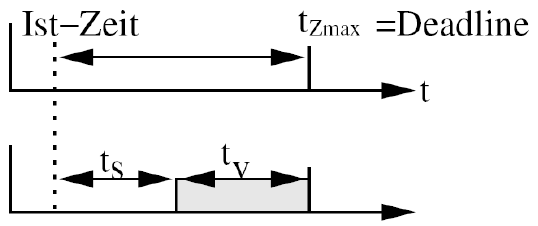
\includegraphics[width=.3\linewidth]{pics/deadline}
		\caption{Deadline-Scheduling}
	\end{center}
\end{figure}
\begin{itemize}
	\item EDF: earliest deadline first
	\item LLF: Least Laxity First
\end{itemize}

\subsection{Prioritätsgesteuert}
\begin{itemize}
	\item Für Realzeitsysteme \underline{geeignet}
	\item Je kürzer die Prozesszeit $t_P$, desto höher die Priorität
	\item I/O bekommt höhere Priorität
\end{itemize}

\subsection{Sporadic Scheduling}
\begin{itemize}
	\item Auslastung $<$ 100\% : Task erhält zusätzliche Rechenzeit
	\item Auslastung = 100\% : Task verletzt Rechtzeitigkeitsbedingung
	\item Replenishment Period T (Prozesszeit)
	\item Initial budget C (Verarbeitungszeit pro Takt)
	\item Priority N
	\item Low Priority L
	\item Maximal number of pending replenishments
\end{itemize}